\documentclass[10pt,aspectratio=169]{beamer}

\usepackage[utf8]{inputenc}
\usepackage[T1]{fontenc}
\usepackage[spanish,es-nodecimaldot]{babel}
\usepackage{amsmath}
\usepackage{amssymb}
\usepackage{booktabs}
\usepackage{graphicx}
\usepackage{xcolor}
\usepackage{tikz}
\usepackage{array}
\usepackage{ragged2e}
\usepackage{hyperref}
\usetikzlibrary{arrows.meta,positioning,calc}

\hypersetup{
    colorlinks=true,
    linkcolor=black,
    urlcolor=black
}

\usetheme{Madrid}
\usecolortheme{default}
\setbeamertemplate{navigation symbols}{}
\setbeamertemplate{headline}{}
\setbeamersize{text margin left=0.7cm,text margin right=0.7cm}
\setbeamertemplate{blocks}[rounded][shadow=false]

\definecolor{ustaNavy}{HTML}{20384F}
\definecolor{ustaSlate}{HTML}{465467}
\definecolor{ustaSoft}{HTML}{F4F6F8}
\definecolor{ustaLine}{HTML}{D9E0E6}
\definecolor{ustaMuted}{HTML}{6D7B8B}

\setbeamercolor{normal text}{fg=ustaSlate,bg=white}
\setbeamercolor{title}{fg=ustaNavy}
\setbeamercolor{frametitle}{fg=ustaNavy,bg=white}
\setbeamercolor{structure}{fg=ustaNavy}
\setbeamercolor{block title}{fg=ustaNavy,bg=ustaSoft}
\setbeamercolor{block body}{fg=ustaSlate,bg=white}
\setbeamercolor{section in toc}{fg=ustaNavy}
\setbeamercolor{author in head/foot}{fg=ustaSlate,bg=ustaSoft}
\setbeamercolor{title in head/foot}{fg=ustaSlate,bg=ustaSoft}
\setbeamercolor{date in head/foot}{fg=ustaSlate,bg=ustaSoft}

\setbeamerfont{title}{size=\Large,series=\bfseries}
\setbeamerfont{frametitle}{size=\large,series=\bfseries}
\setbeamerfont{block title}{series=\bfseries}

\setbeamertemplate{itemize item}{\color{ustaNavy}\scriptsize$\blacksquare$}
\setbeamertemplate{itemize subitem}{\color{ustaNavy}\tiny$\blacksquare$}

\addtobeamertemplate{frametitle}{}{%
    \vspace{-0.35em}
    \hspace*{0.01\paperwidth}{\color{ustaLine}\rule{0.96\paperwidth}{0.45pt}}
}

\setbeamertemplate{footline}{
    \leavevmode
    \hbox{
        \begin{beamercolorbox}[wd=.28\paperwidth,ht=2.85ex,dp=1.2ex,leftskip=0.8em]{author in head/foot}
            \footnotesize Natalia Zárate
        \end{beamercolorbox}
        \begin{beamercolorbox}[wd=.22\paperwidth,ht=2.85ex,dp=1.2ex,center]{title in head/foot}
            \footnotesize Junio 2026
        \end{beamercolorbox}
        \begin{beamercolorbox}[wd=.32\paperwidth,ht=2.85ex,dp=1.2ex,center]{date in head/foot}
            \footnotesize USTA Bogotá · Estadística
        \end{beamercolorbox}
        \begin{beamercolorbox}[wd=.18\paperwidth,ht=2.85ex,dp=1.2ex,rightskip=0.8em,right]{date in head/foot}
            \footnotesize \insertframenumber{} / \inserttotalframenumber
        \end{beamercolorbox}
    }
}

\newcommand{\softcard}[2]{
    \begin{beamercolorbox}[rounded=true,sep=0.9em,wd=\linewidth]{block body}
        {\color{ustaNavy}\textbf{#1}}\\[0.25em]
        #2
    \end{beamercolorbox}
}

\title[IBNR y Chain-Ladder robusto]{Estimación del IBNR con Chain-Ladder robusto\\bajo datos contaminados}
\subtitle{Proyecto de grado}
\author[Natalia Zárate]{Natalia Zárate}
\institute[USTA Bogotá]{
Facultad de Estadística\\
Universidad Santo Tomás, Bogotá\\[0.2cm]
\small Práctica en Advisory -- Financial Risk Management\\
\small KPMG Advisory, Tax \& Legal S.A.S.
}
\date[Junio 2026]{Junio de 2026}

\titlegraphic{
    \vspace{0.25cm}
    \IfFileExists{figuras/logo_usta.png}{
\includegraphics[height=1.1cm]{figuras/logo_usta.png}}{}%
    \hspace{1.1cm}
    \IfFileExists{figuras/logo_kpmg.png}{
\includegraphics[height=0.75cm]{figuras/logo_kpmg.png}}{}%
}

\begin{document}

\begin{frame}
    \titlepage
\end{frame}

\begin{frame}{¿Qué es el IBNR y por qué importa?}
    \begin{columns}[T]
        \column{0.42\textwidth}
        \begin{itemize}
            \item El IBNR corresponde a siniestros ya ocurridos pero no observados completamente al momento de estimar
            \item En el triángulo de desarrollo, esa parte futura debe proyectarse con información incompleta
            \item Si la región observada tiene valores atípicos, la reserva puede quedar sesgada
        \end{itemize}

        \vspace{0.35cm}
        \softcard{Definición operativa}{
            \[
            IBNR^{\text{real}}=\sum_{(i,j)\in\mathcal{F}} X_{ij}
            \]
            donde $\mathcal{F}$ representa la zona futura no observada del triángulo.
        }

        \column{0.58\textwidth}
        \centering
        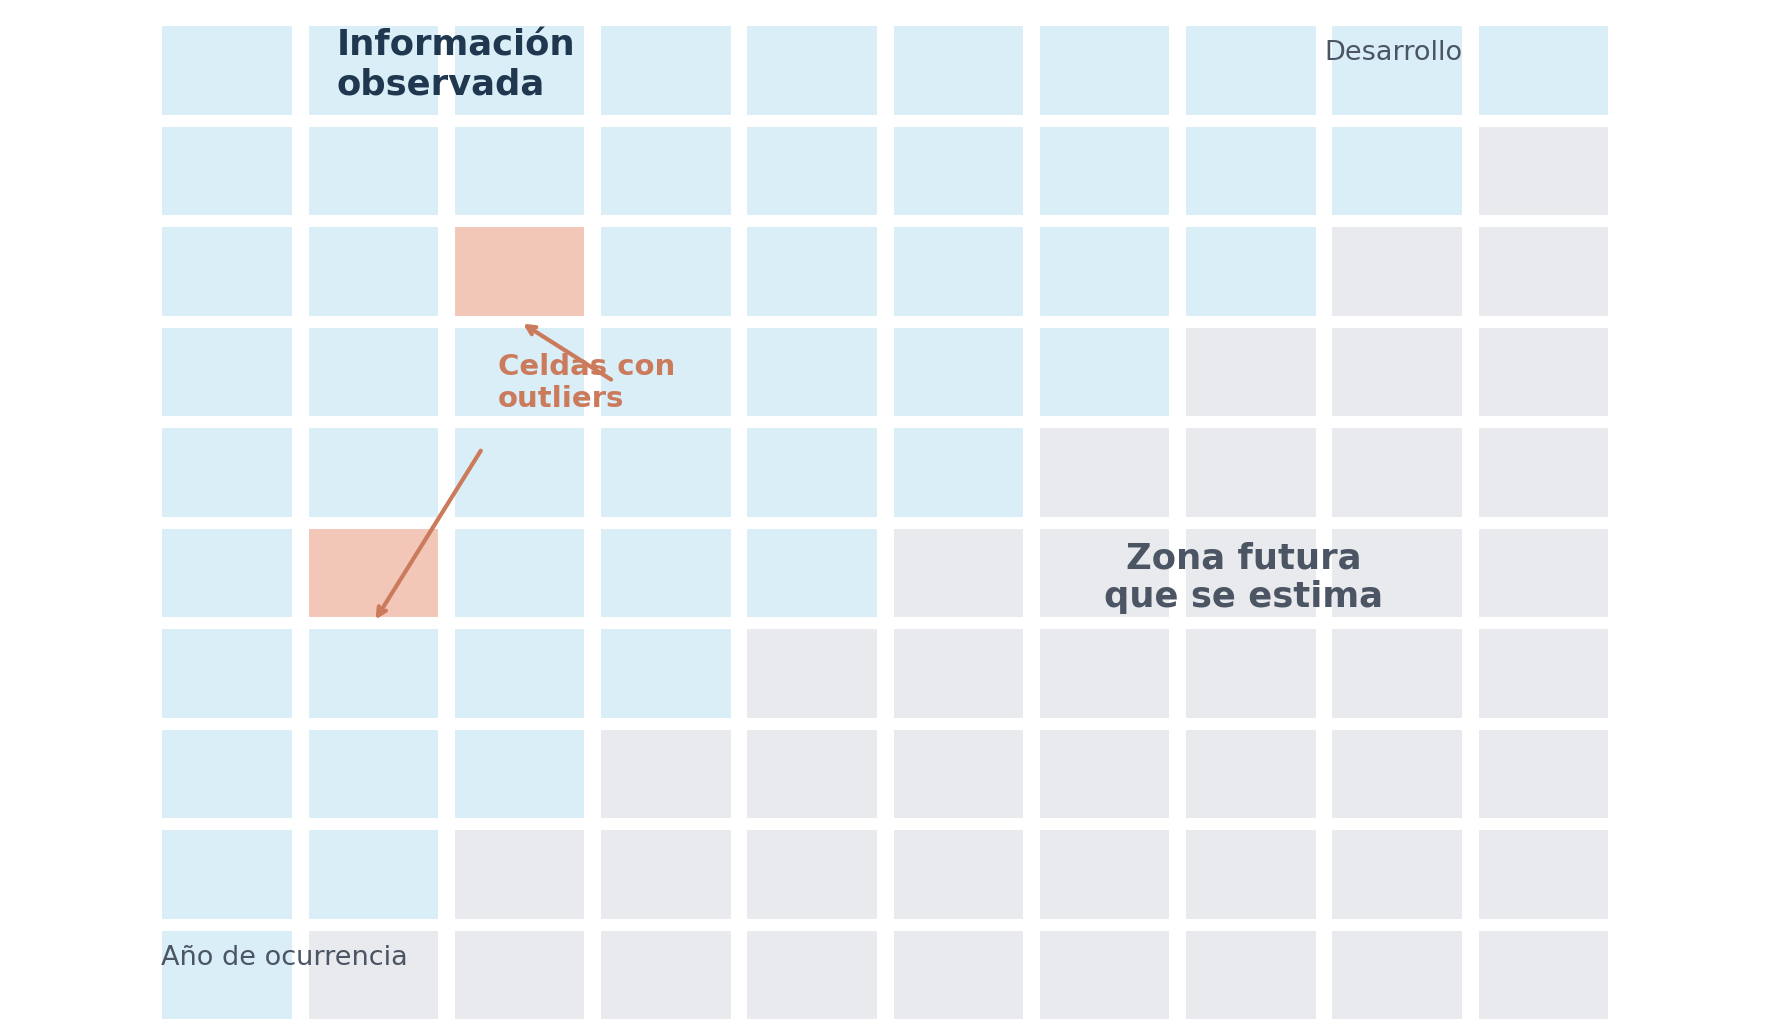
\includegraphics[width=\linewidth]{figuras/triangulo_ibnr.png}
    \end{columns}
\end{frame}

\begin{frame}{Antecedentes y vacío del estudio}
    \centering
    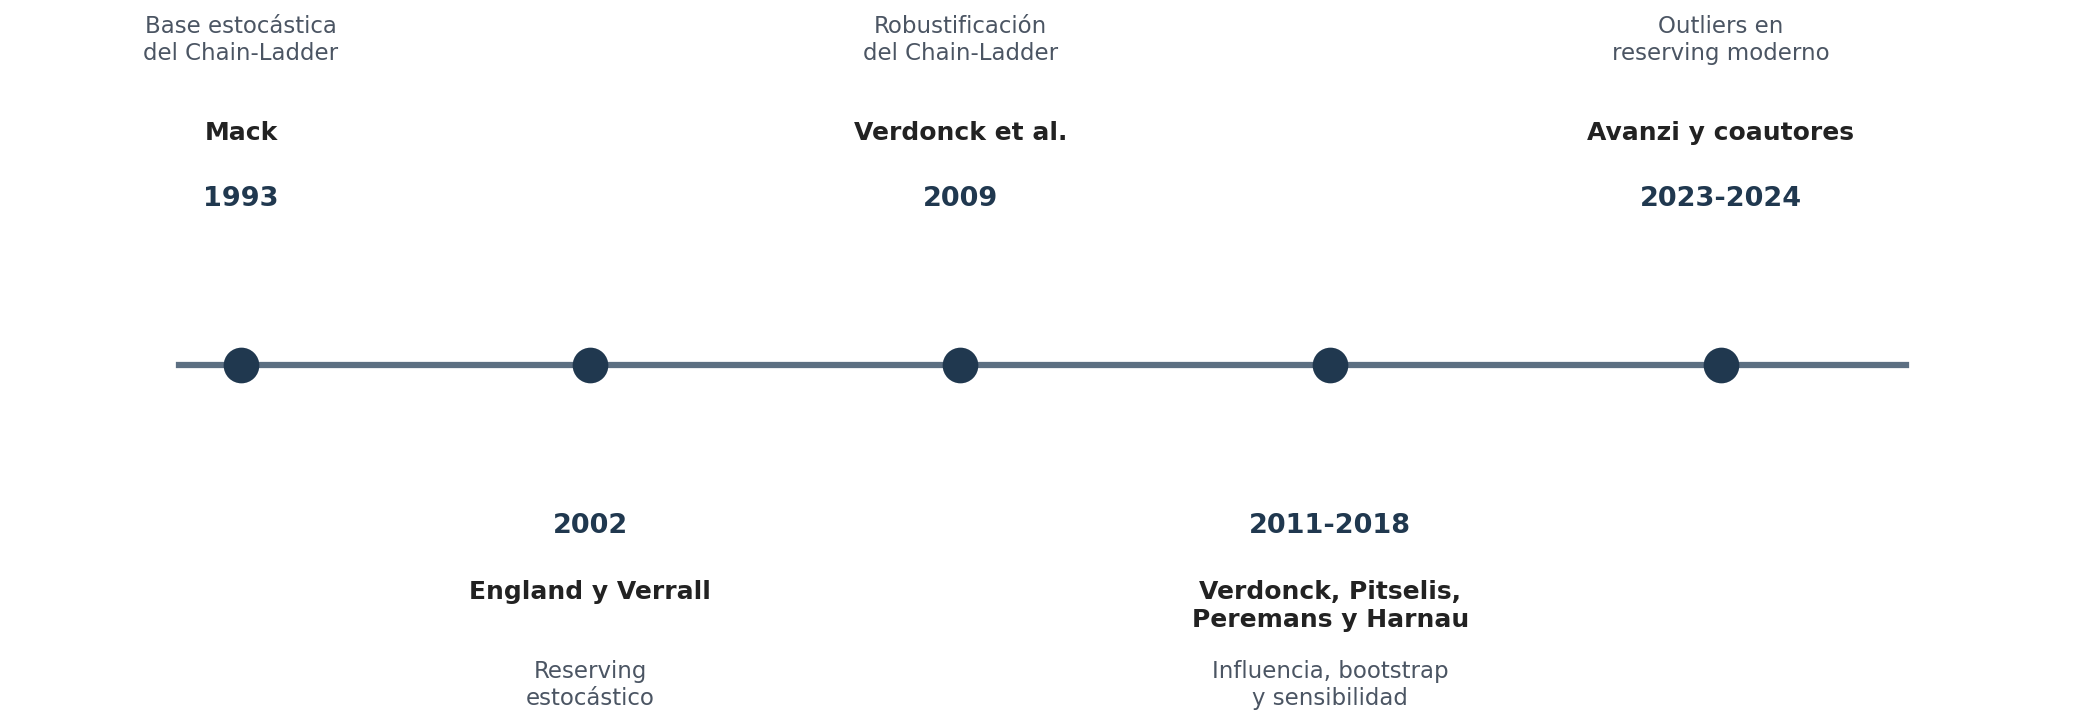
\includegraphics[width=0.95\linewidth]{figuras/linea_tiempo_antecedentes.png}

    \vspace{0.25cm}
    \softcard{Vacío que aborda este proyecto}{
        La literatura reconoce la sensibilidad del Chain-Ladder frente a outliers, pero no toda robustificación mejora del mismo modo. Por eso se comparan varias alternativas bajo un diseño de simulación controlado.
    }
\end{frame}

\begin{frame}{Pregunta de investigación}
    \begin{columns}[T]
        \column{0.58\textwidth}
        \softcard{Pregunta central}{
            ¿Bajo qué combinaciones de proporción, magnitud y ubicación de la contaminación las variantes robustas superan al método Chain-Ladder clásico en la estimación del IBNR?
        }

        \vspace{0.45cm}
        \softcard{Interpretación estadística}{
            La comparación se hace escenario por escenario, manteniendo los mismos triángulos simulados y evaluando si cambia el error de estimación y la estabilidad entre réplicas.
        }

        \column{0.42\textwidth}
        \softcard{Escenario de contaminación}{
            \[
            s=(p,m,u)
            \]
            \begin{itemize}
                \item $p$: proporción contaminada
                \item $m$: magnitud del outlier
                \item $u$: ubicación en la región observada
            \end{itemize}
        }
    \end{columns}
\end{frame}

\begin{frame}{Objetivo e hipótesis de trabajo}
    \begin{columns}[T]
        \column{0.5\textwidth}
        \softcard{Objetivo general}{
            Comparar el método Chain-Ladder clásico y tres variantes robustas para estimar el IBNR bajo escenarios controlados de contaminación.
        }

        \vspace{0.4cm}
        \softcard{Variable de respuesta}{
            Para cada método $k$ y escenario $s$ se resume el desempeño mediante
            \[
            L_{k,s}=(\text{sesgo},\ \text{RMSE},\ \text{MAPE},\ \text{DE})
            \]
        }

        \column{0.5\textwidth}
        \softcard{Hipótesis de trabajo}{
            Si la contaminación aumenta, el método clásico comete más error, mientras que al menos una variante robusta mantiene menor error y estimaciones más estables.
        }

        \vspace{0.4cm}
        \softcard{Lectura matemática}{
            Si $p$ y $m$ aumentan, entonces
            \[
            RMSE_{\text{CL},s}\uparrow
            \]
            y para al menos una variante robusta $r$ se espera que
            \[
            RMSE_{r,s}<RMSE_{\text{CL},s},\qquad DE_{r,s}<DE_{\text{CL},s}
            \]
        }
    \end{columns}
\end{frame}

\begin{frame}{Metodología general}
    \centering
    \begin{tikzpicture}[
        node distance=0.6cm and 0.38cm,
        box/.style={draw=ustaLine, rounded corners=2pt, fill=ustaSoft, minimum height=1cm, text width=2.55cm, align=center, font=\small},
        arrow/.style={-{Latex[length=2.5mm]}, draw=ustaNavy, line width=0.85pt}
    ]
        \node[box] (configuracion) {Configurar\\el experimento};
        \node[box, right=of configuracion] (simulate) {Simular\\triángulos completos};
        \node[box, right=of simulate] (hide) {Ocultar\\la zona futura};
        \node[box, below=of simulate] (contaminate) {Contaminar\\la región observada};
        \node[box, left=of contaminate] (metodos) {Aplicar\\cuatro métodos};
        \node[box, right=of contaminate] (compare) {Comparar\\error y estabilidad};

        \draw[arrow] (configuracion) -- (simulate);
        \draw[arrow] (simulate) -- (hide);
        \draw[arrow] (hide) |- (contaminate);
        \draw[arrow] (contaminate) -- (metodos);
        \draw[arrow] (contaminate) -- (compare);
    \end{tikzpicture}

    \vspace{0.45cm}
    \begin{columns}[T]
        \column{0.33\textwidth}
        \softcard{Generación base}{
            \[
            X_{ij}\sim\text{Gamma}(\mu_{ij},\phi)
            \]
            con sensibilidad posterior bajo un esquema Lognormal.
        }

        \column{0.33\textwidth}
        \softcard{Contaminación}{
            Solo se modifica la región observada para no alterar el IBNR real de la zona futura.
        }

        \column{0.33\textwidth}
        \softcard{Comparación}{
            Todos los métodos se evalúan sobre los mismos triángulos simulados.
        }
    \end{columns}
\end{frame}

\begin{frame}{Diseño experimental}
    \begin{columns}[T]
        \column{0.34\textwidth}
        \softcard{Base del estudio}{
            \begin{itemize}
                \item Triángulos 10 $\times$ 10
                \item 1000 réplicas por escenario
                \item Gamma como caso base
                \item Lognormal como sensibilidad
            \end{itemize}
        }

        \vspace{0.4cm}
        \softcard{Escenarios}{
            1 escenario limpio y 27 escenarios contaminados definidos por
            \[
            (p,m,u)
            \]
        }

        \column{0.66\textwidth}
        \centering
        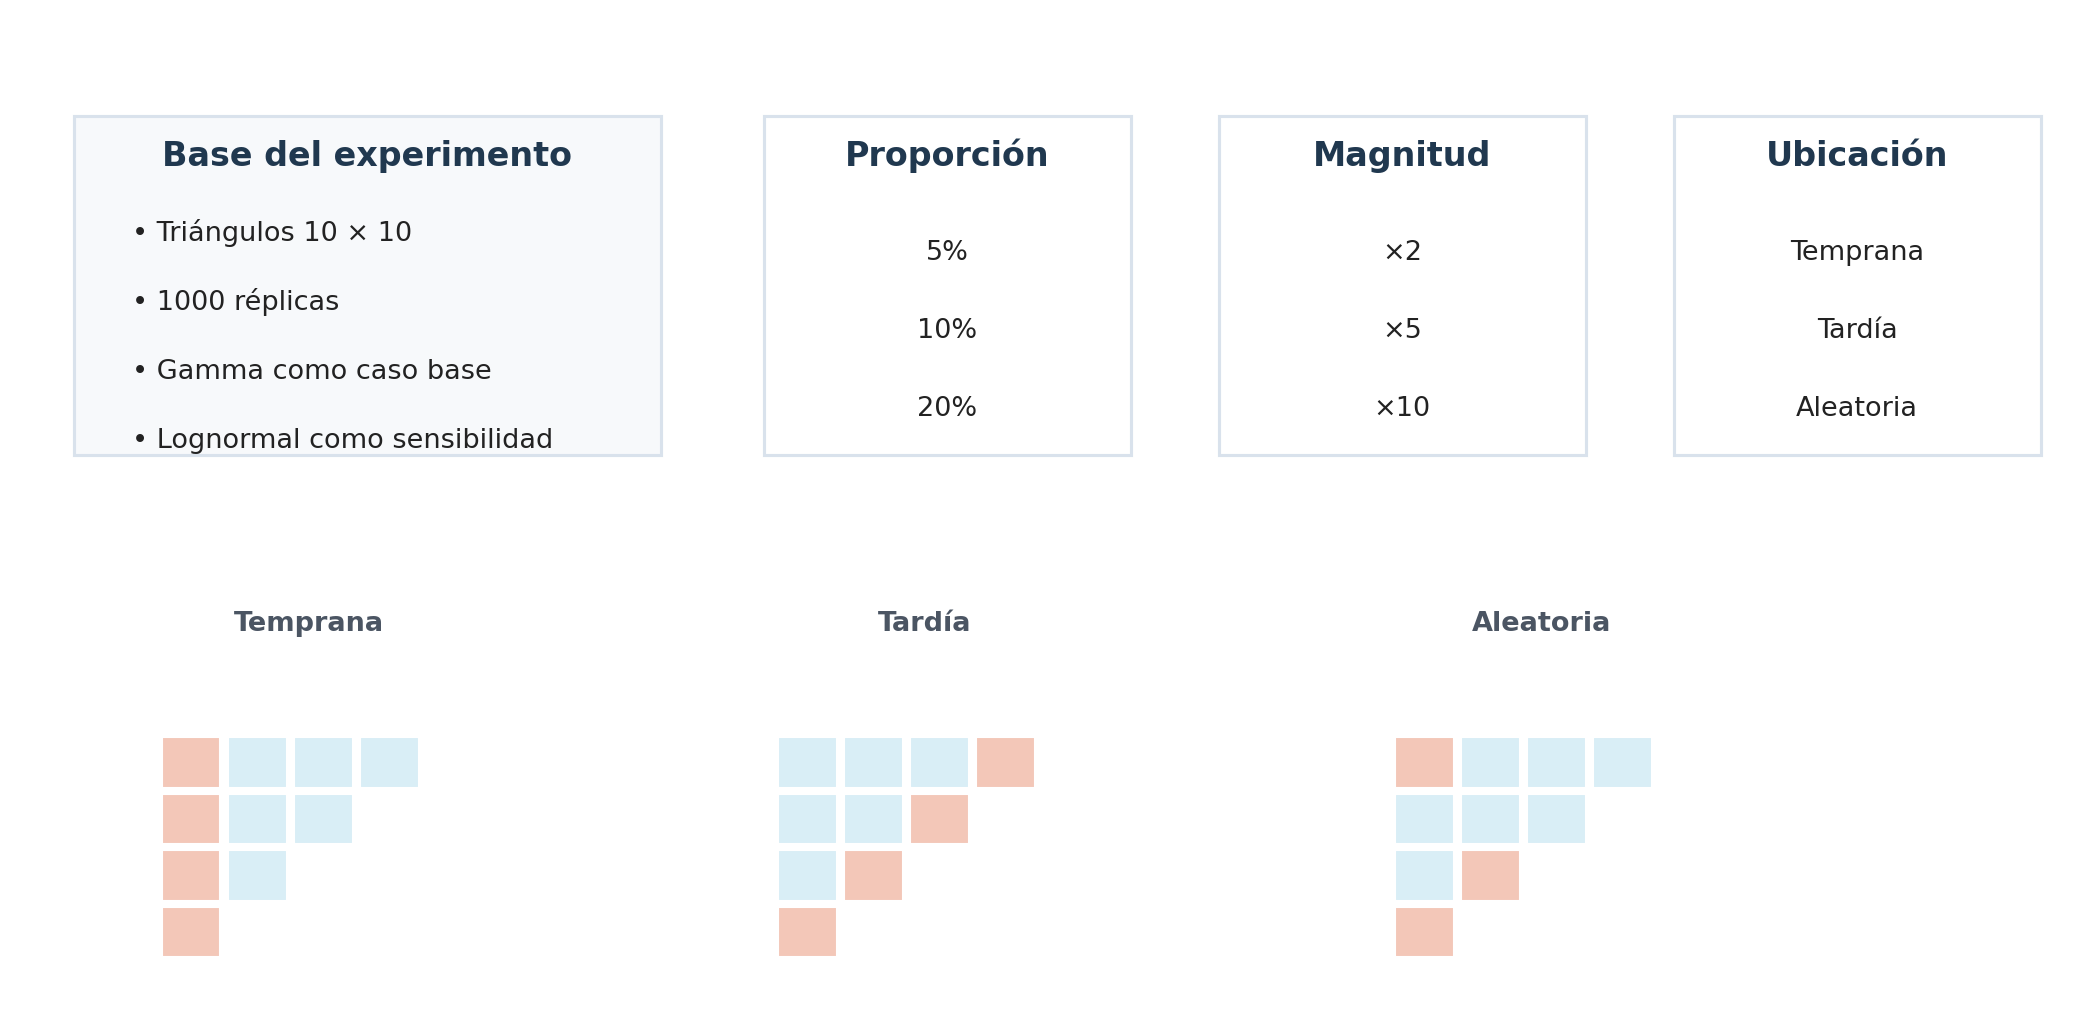
\includegraphics[width=\linewidth]{figuras/diseno_experimental.png}
    \end{columns}
\end{frame}

\begin{frame}{Validación del simulador}
    \begin{columns}[T]
        \column{0.57\textwidth}
        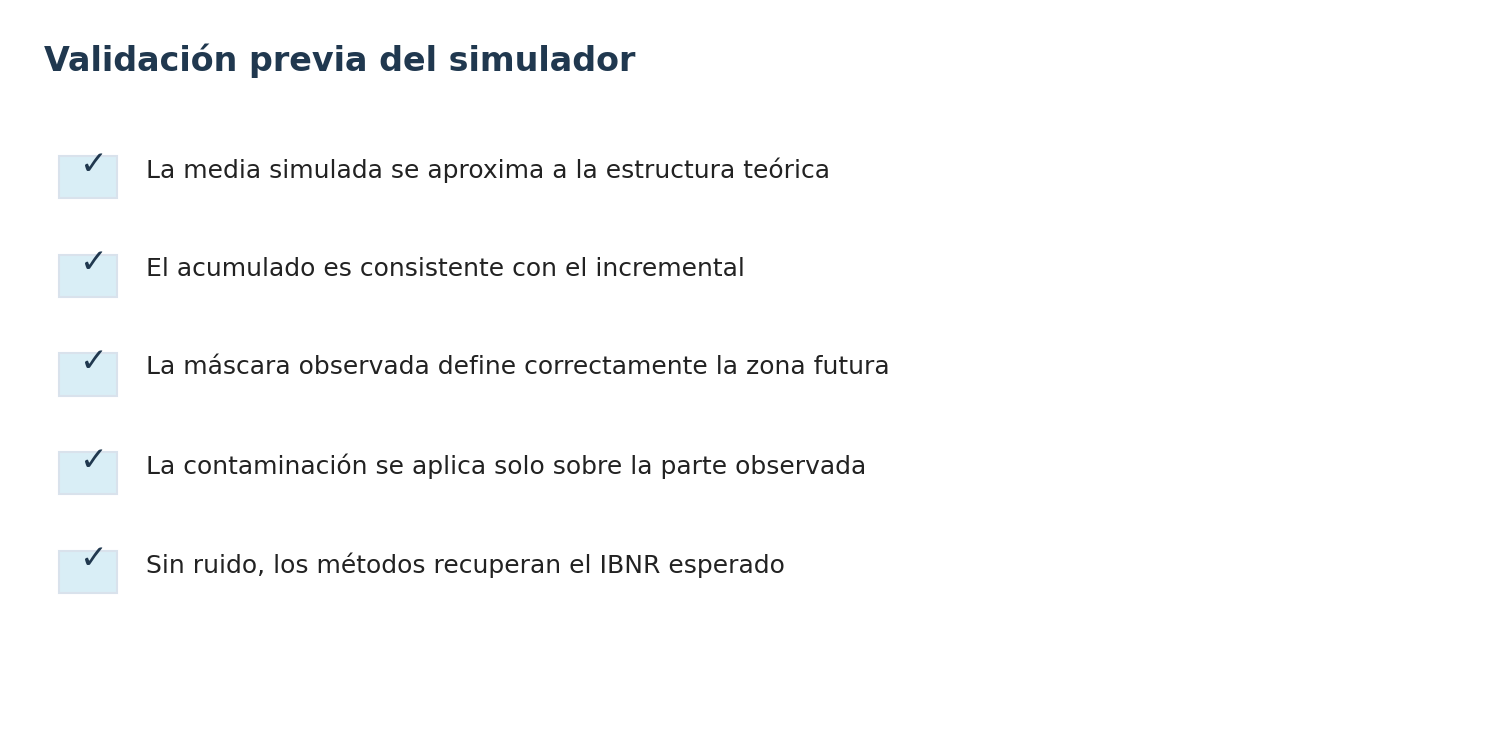
\includegraphics[width=\linewidth]{figuras/lista_validacion.png}

        \column{0.43\textwidth}
        \softcard{Verificaciones realizadas}{
            \begin{itemize}
                \item Coherencia entre medias teóricas y simuladas
                \item Consistencia entre incremental y acumulado
                \item Definición correcta de la máscara observada
                \item Recuperación del IBNR esperado en un caso sin ruido
            \end{itemize}
        }

        \vspace{0.35cm}
        \softcard{Papel dentro del estudio}{
            Esta etapa verifica que el experimento compare métodos y no errores de implementación del simulador.
        }
    \end{columns}
\end{frame}

\begin{frame}{Métodos y métricas de comparación}
    \centering
    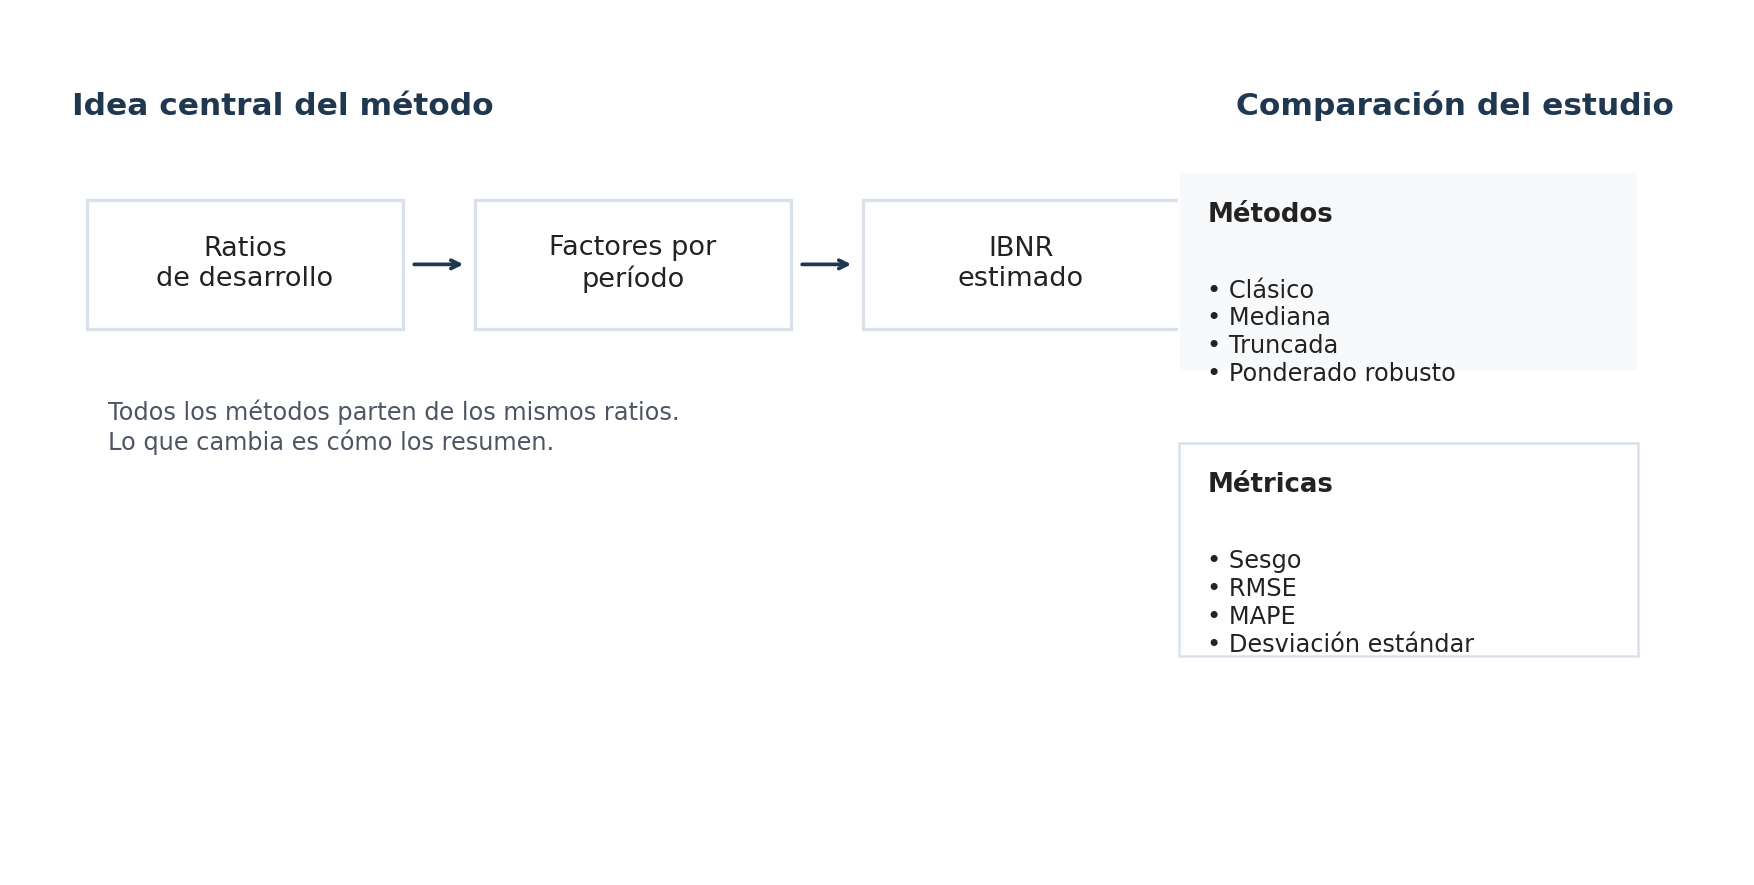
\includegraphics[width=0.92\linewidth]{figuras/metodos_metricas.png}

    \vspace{0.35cm}
    \begin{columns}[T]
        \column{0.5\textwidth}
        \softcard{Métodos}{
            Clásico, mediana, media truncada y ponderado robusto.
        }

        \column{0.5\textwidth}
        \softcard{Criterio principal}{
            El contraste principal se hace con RMSE y se complementa con MAPE, sesgo y desviación estándar entre réplicas.
        }
    \end{columns}
\end{frame}

\begin{frame}{Resultados principales}
    \begin{columns}[T]
        \column{0.56\textwidth}
        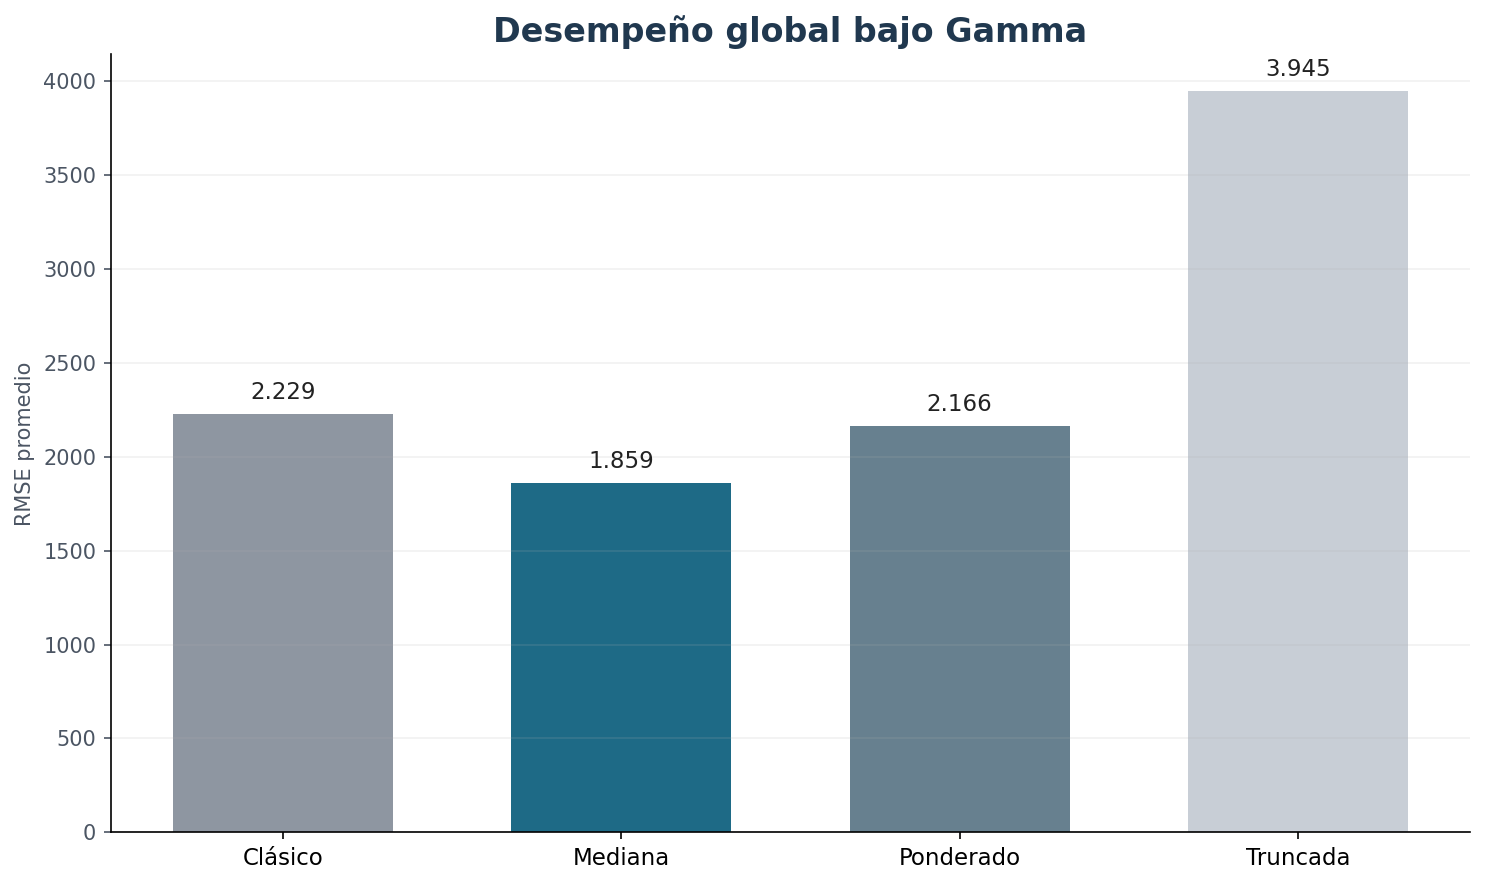
\includegraphics[width=\linewidth]{figuras/rmse_global.png}

        \column{0.44\textwidth}
        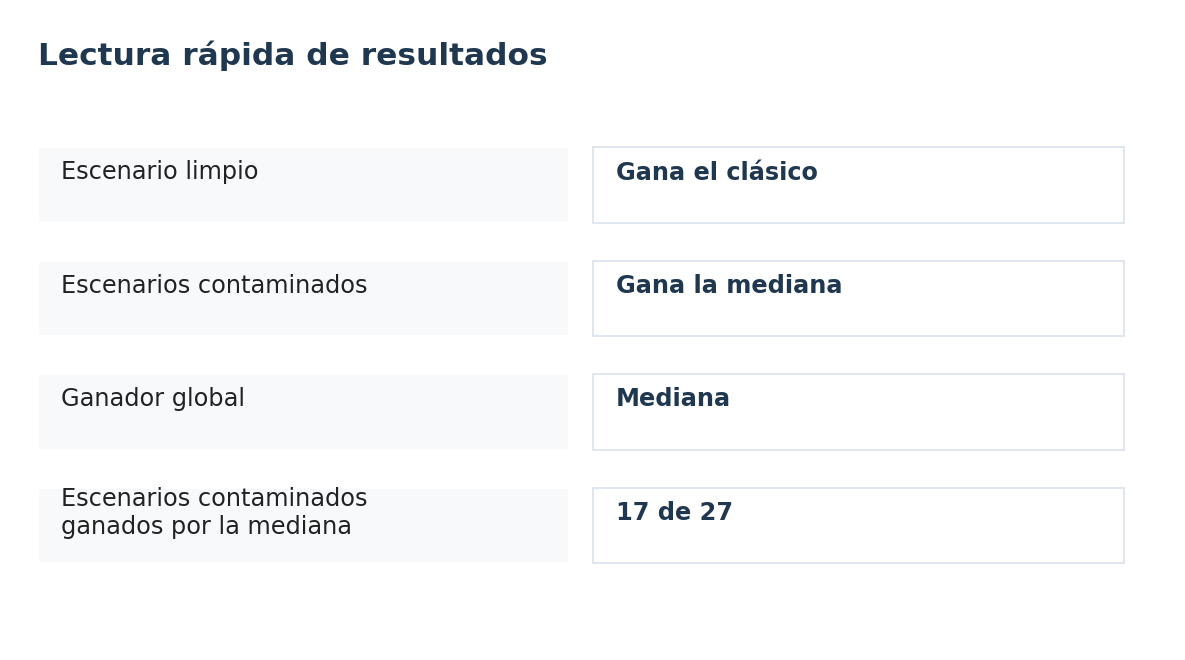
\includegraphics[width=\linewidth]{figuras/resumen_resultado_global.png}
    \end{columns}

    \vspace{0.25cm}
    \softcard{Hallazgo central}{
        El método clásico gana en el escenario limpio, pero la mediana se convierte en la alternativa más consistente cuando la contaminación deja de ser leve.
    }
\end{frame}

\begin{frame}{¿Cuándo gana cada método?}
    \begin{columns}[T]
        \column{0.62\textwidth}
        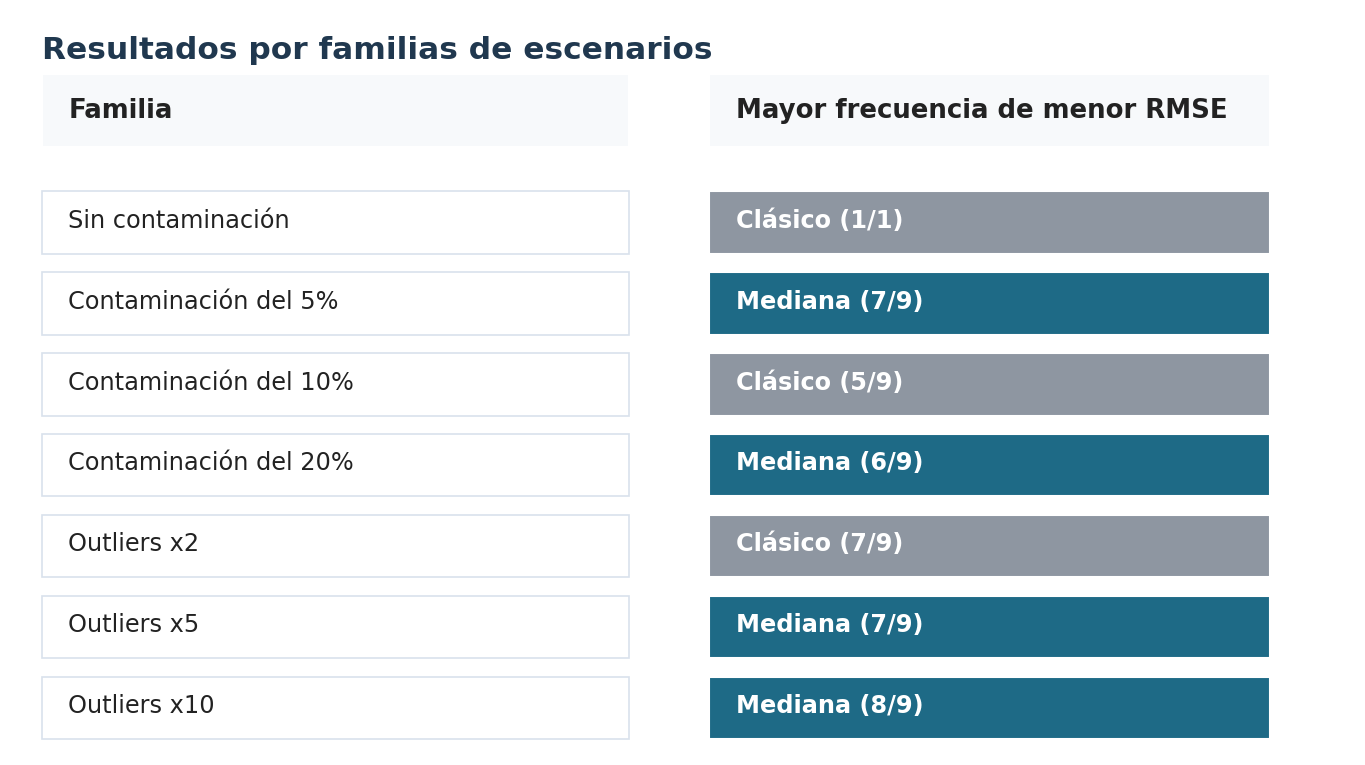
\includegraphics[width=\linewidth]{figuras/familias_resultados.png}

        \column{0.38\textwidth}
        \softcard{Patrones por familias}{
            \begin{itemize}
                \item Escenario limpio: ventaja del clásico
                \item La mediana lidera el RMSE promedio en todas las familias contaminadas
                \item El clásico conserva más victorias en 10\%, outliers $\times 2$ y contaminación temprana
                \item Tardía y aleatoria: escenarios más favorables para la mediana
            \end{itemize}
        }
    \end{columns}
\end{frame}

\begin{frame}{Sensibilidad distribucional}
    \begin{columns}[T]
        \column{0.56\textwidth}
        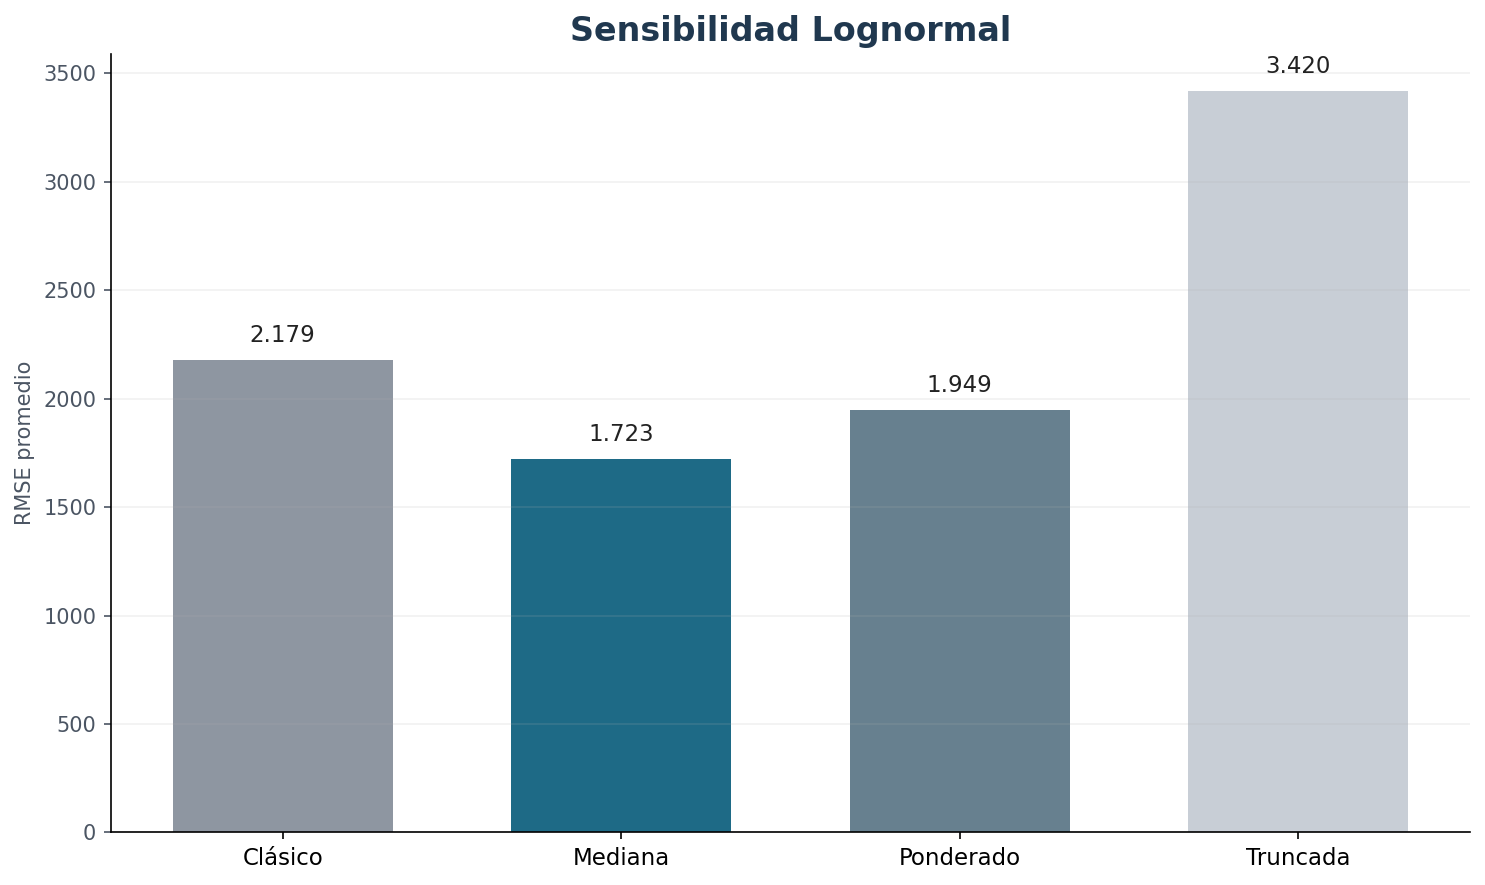
\includegraphics[width=\linewidth]{figuras/rmse_lognormal.png}

        \column{0.44\textwidth}
        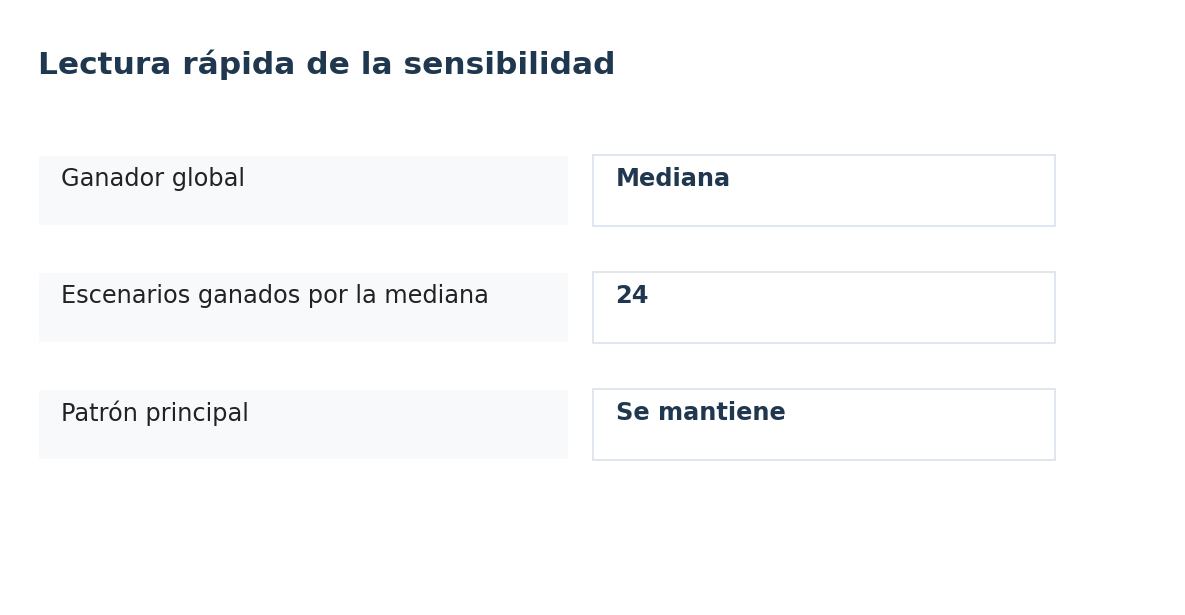
\includegraphics[width=\linewidth]{figuras/resumen_lognormal.png}
    \end{columns}

    \vspace{0.25cm}
    \softcard{Lectura}{
        La sensibilidad bajo Lognormal no cambia la conclusión principal del estudio. La mediana sigue liderando el desempeño global.
    }
\end{frame}

\begin{frame}{Conclusiones}
    \begin{columns}[T]
        \column{0.5\textwidth}
        \softcard{Conclusión 1}{
            El método clásico conserva eficiencia cuando la contaminación es nula o débil.
        }

        \vspace{0.35cm}
        \softcard{Conclusión 2}{
            La mediana es la variante más consistente cuando la contaminación aumenta en proporción o magnitud.
        }

        \column{0.5\textwidth}
        \softcard{Conclusión 3}{
            La media truncada y el ponderado no superan de forma general a la mediana en este diseño.
        }

        \vspace{0.35cm}
        \softcard{Conclusión 4}{
            La sensibilidad Lognormal mantiene el patrón principal de resultados.
        }
    \end{columns}

    \vspace{0.35cm}
    \centering
    \textbf{\color{ustaNavy}Respuesta central:} la robustificación sí mejora la estimación del IBNR, pero no en todos los escenarios ni con la misma intensidad.
\end{frame}

\begin{frame}{Discusión, alcance y trabajo futuro}
    \begin{columns}[T]
        \column{0.5\textwidth}
        \softcard{Alcance}{
            \begin{itemize}
                \item Estudio de simulación sobre triángulos agregados
                \item Comparación reproducible entre cuatro métodos
                \item Contaminación positiva y controlada
            \end{itemize}
        }

        \vspace{0.35cm}
        \softcard{Aporte}{
            El proyecto no propone un método nuevo. Identifica con claridad cuándo una robustificación simple mejora al Chain-Ladder clásico.
        }

        \column{0.5\textwidth}
        \softcard{Limitaciones}{
            \begin{itemize}
                \item No trabaja con una cartera real
                \item No incorpora bootstrap robusto completo
                \item No aborda marcos multivariados o micro-level
            \end{itemize}
        }

        \vspace{0.35cm}
        \softcard{Trabajo futuro}{
            Datos reales, inferencia robusta y extensiones multivariadas o a nivel individual del siniestro.
        }
    \end{columns}
\end{frame}

\begin{frame}{Bibliografía clave}
    \scriptsize
    \begin{columns}[T]
        \column{0.5\textwidth}
        \textbf{\color{ustaNavy}Base actuarial y estocástica}
        \begin{itemize}
            \item Mack, T. (1993). \textit{Distribution-Free Calculation of the Standard Error of Chain-Ladder Reserve Estimates}.
            \item England, P. D. y Verrall, R. J. (2002). \textit{Stochastic Claims Reserving in General Insurance}.
            \item Wüthrich, M. V. y Merz, M. (2008). \textit{Stochastic Claims Reserving Methods in Insurance}.
            \item Harnau, J. (2018). \textit{Misspecification Tests for Log-Normal and Over-Dispersed Poisson Chain-Ladder Models}.
        \end{itemize}

        \column{0.5\textwidth}
        \textbf{\color{ustaNavy}Robustez y outliers}
        \begin{itemize}
            \item Verdonck, T., Van Wouwe, M. y Dhaene, J. (2009). \textit{A Robustification of the Chain-Ladder Method}.
            \item Verdonck, T. y Debruyne, M. (2011). \textit{The Influence of Individual Claims on the Chain-Ladder Estimates}.
            \item Pitselis, G., Grigoriadou, V. y Badounas, I. (2015). \textit{Robust Loss Reserving in a Log-Linear Model}.
            \item Peremans, K., Van Aelst, S. y Verdonck, T. (2018). \textit{A Robust General Multivariate Chain Ladder Method}.
            \item Avanzi, B., Richman, R. y Wong, B. (2023). \textit{Detection and Treatment of Outliers for Multivariate Robust Loss Reserving}.
            \item Avanzi, B., Lavender, A., Taylor, G. y Wong, B. (2024). \textit{On the Impact of Outliers in Loss Reserving}.
        \end{itemize}
    \end{columns}
\end{frame}

\begin{frame}
    \centering
    {\Large\color{ustaNavy}\textbf{Gracias}}\\[0.45cm]
    Preguntas y comentarios
\end{frame}

\end{document}
